%% 
%% Copyright 2007-2019 Elsevier Ltd
%% 
%% This file is part of the 'Elsarticle Bundle'.
%% ---------------------------------------------
%% 
%% It may be distributed under the conditions of the LaTeX Project Public
%% License, either version 1.2 of this license or (at your option) any
%% later version.  The latest version of this license is in
%%    http://www.latex-project.org/lppl.txt
%% and version 1.2 or later is part of all distributions of LaTeX
%% version 1999/12/01 or later.
%% 
%% The list of all files belonging to the 'Elsarticle Bundle' is
%% given in the file `manifest.txt'.
%% 
%% Template article for Elsevier's document class `elsarticle'
%% with harvard style bibliographic references

%\documentclass[preprint,12pt,authoryear]{elsarticle}

%% Use the option review to obtain double line spacing
%% \documentclass[authoryear,preprint,review,12pt]{elsarticle}

%% Use the options 1p,twocolumn; 3p; 3p,twocolumn; 5p; or 5p,twocolumn
%% for a journal layout:
%% \documentclass[final,1p,times,authoryear]{elsarticle}
%% \documentclass[final,1p,times,twocolumn,authoryear]{elsarticle}
%% \documentclass[final,3p,times,authoryear]{elsarticle}
\documentclass[final,3p,times,twocolumn,numbers]{elsarticle}
%% \documentclass[final,5p,times,authoryear]{elsarticle}
%% \documentclass[final,5p,times,twocolumn,authoryear]{elsarticle}

%% For including figures, graphicx.sty has been loaded in
%% elsarticle.cls. If you prefer to use the old commands
%% please give \usepackage{epsfig}

%% The amssymb package provides various useful mathematical symbols
\usepackage{amssymb}
%% The amsthm package provides extended theorem environments
\usepackage{amsthm}

\usepackage{mhchem}
\usepackage{xcolor}

%% The lineno packages adds line numbers. Start line numbering with
%% \begin{linenumbers}, end it with \end{linenumbers}. Or switch it on
%% for the whole article with \linenumbers.
%% \usepackage{lineno}

\journal{Applied Energy}

\begin{document}

\begin{frontmatter}

%% Title, authors and addresses

%% use the tnoteref command within \title for footnotes;
%% use the tnotetext command for theassociated footnote;
%% use the fnref command within \author or \address for footnotes;
%% use the fntext command for theassociated footnote;
%% use the corref command within \author for corresponding author footnotes;
%% use the cortext command for theassociated footnote;
%% use the ead command for the email address,
%% and the form \ead[url] for the home page:
 \title{Validating the long-term electricity market model ElecSim}
% \tnotetext[label1]{}
 \author{Alexander J. M. Kell}
 \ead{a.kell2@newcastle.ac.uk}
% \ead[url]{home page}
% \fntext[label2]{}
% \cortext[cor1]{}
% \address{Address\fnref{label3}}
% \fntext[label3]{}

%\title{Validating a long-term electricity market model}

%% use optional labels to link authors explicitly to addresses:
%% \author[label1,label2]{}
%% \address[label1]{}
%% \address[label2]{}

\author{A. Stephen McGough, Matthew Forshaw}

\address{School of Computing, Newcastle University, Newcastle-upon-Tyne, United Kingdom}

\begin{abstract}
%% Text of abstract

\end{abstract}
%
%%%Graphical abstract
%\begin{graphicalabstract}
%\includegraphics{grabs}
%Hello test
%\end{graphicalabstract}
%
%%%Research highlights
%\begin{highlights}
%\item Validating a model
%\item Optimisation
%\item Scenario modelling
%\end{highlights}

\begin{keyword}
%% keywords here, in the form: keyword \sep keyword
Long-term energy modelling \sep model validation \sep Machine learning \sep Optimization
%% PACS codes here, in the form: \PACS code \sep code

%% MSC codes here, in the form: \MSC code \sep code
%% or \MSC[2008] code \sep code (2000 is the default)

\end{keyword}

\end{frontmatter}

%% \linenumbers

%% main text
\section{Introduction}
\label{sec:intro}


To limit the effects of climate change, a transition from a fossil-fuel based system to one based on low-carbon, renewable energy is required. The report by the Intergovernmental Panel on Climate Change detailed that reaching and sustaining zero global anthropogenic \ce{CO2} would halt anthropogenic global warming on multi-decadal time scales \cite{Masson-Delmotte2018}. 

The Paris Agreement was a declaration signed in 2015 by 195 state parties to plan and regularly report on the contribution made to mitigate global warming \cite{May2002}. Based on this commitment, policy makers require quantitive advice on interventions to aid in the mitigation of climate change and limit global average temperatures to well below 2$^{\circ}$C. 

The decarbonization of electricity generation is of strategic importance for this goal, due to the fact that low-carbon electricity can enable reductions in \ce{CO2} emissions in industry, transport and building sectors~\cite{Salas2017}. 

However, there remain a number of uncertainties in the technological transition to a low-carbon energy supply. Examples of these uncertainties are investor behaviour, future prices of electricity generation and storage, domestic and international policy, energy efficiency and electricity demand. To successfully create effective policies an increase in understanding of these uncertainties and how they interact is required.

Energy modelling is a method that allows policy makers to increase their understanding of policy decision outcomes under a wide range of scenarios. Agent-based modelling (ABM) is a simulation technique that allows for heterogeneous agents to interact and can lead to effects on the aggregated level of the total system, a phenomenon called ``emergence'' \cite{EpsteinJoshuaM.author.GSSS}. Traditional models for analysing electricity systems, such as centralised optimisation models do not account for the heterogeneous nature of electricity investors and are, to some extent, based on obsolete assumptions~\cite{Ringler2016}.

In this paper we motivate that agent-based models are a valid way of complimenting existing models to provide advice to decision makers. We show that the model ElecSim \cite{Kell} can be validated for a 5 year period, starting from the year 2013 until the year 2018, with a mean absolute percentage error of {\color{red} XX\%} and a standard deviation of {\color{red}XX}. Similarly to Nahmmacher \textit{et al.} we demonstrate how clustering of multiple relevant time series such as electricity demand, solar irradiance and wind speed can reduce computational time by selecting representative days~\cite{Nahmmacher2016}. However, distinctly to Nahmacher \textit{et al.} we use a K-means clustering approach \cite{forgy65} as opposed to a hierarchical clustering algorithm described by Ward \cite{doi:10.1080/01621459.1963.10500845}.

We use a genetic algorithm approach to find an optimal set of price curves predicted by generation companies (GenCos) that  adequately model observed investment behaviour in the real-life electricity market in the United Kingdom. However, similar techniques can be employed for other countries of various sizes. We accurately capture the transitional dynamics of the electricity mix in the United Kingdom as shown in Figure \ref{uk_historical_mix}, where there was an $\sim88\%$ drop in coal use, $\sim44\%$ increase in Combined Cycle Gas Turbines (CCGT) and a $\sim111\% $ increase in wind energy.


\begin{figure}
\centering
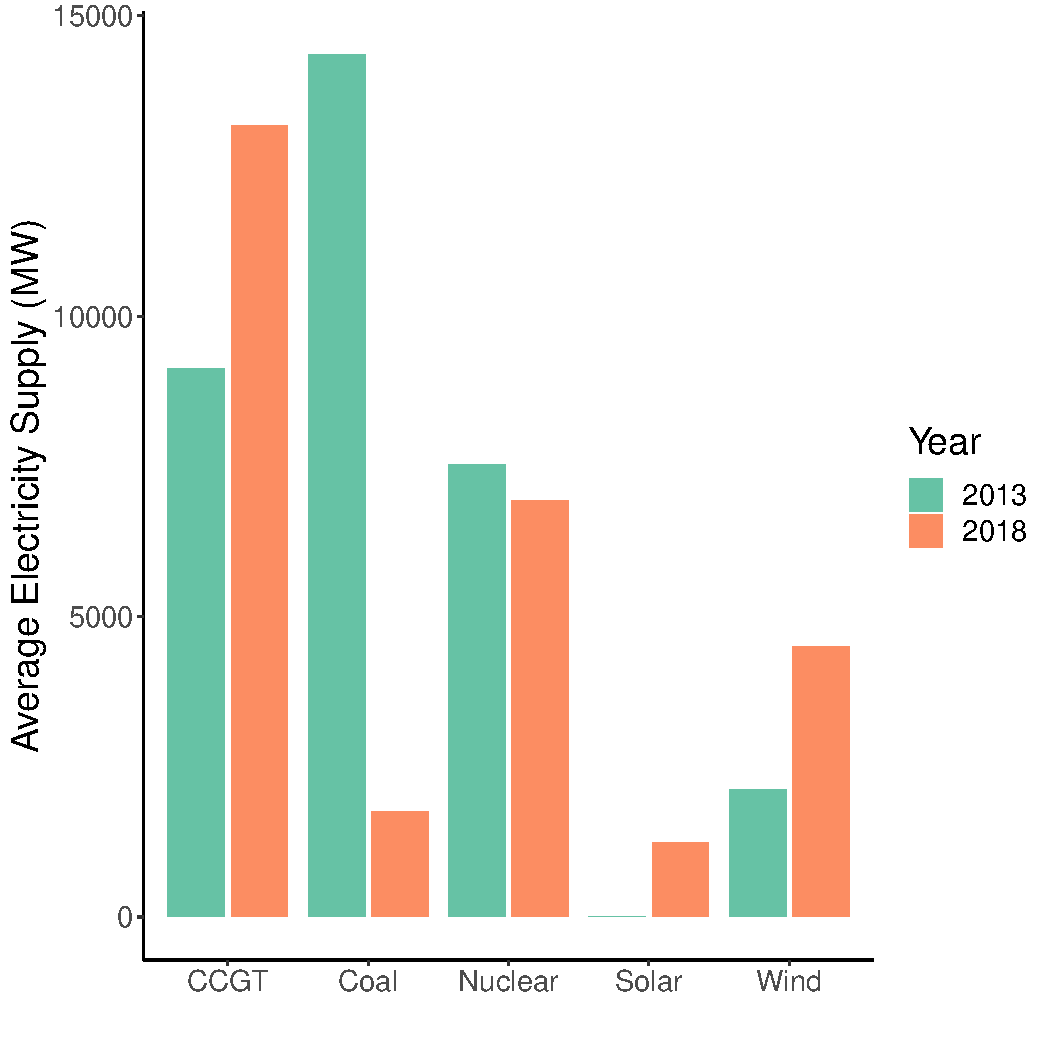
\includegraphics[width=0.46\textwidth]{figures/introduction/uk_historical_mix.pdf}
\label{uk_historical_mix}
\caption{Electricity generation transition from 2013 to 2018 in the United Kingdom.}
\end{figure}


\begin{itemize}
	\item Energy systems modelling to help transition to low-carbon energy systems (Paris Agreement)
	\item Application of quantitive analysis to policy
	\item Use of agent-based models to model heterogeneous actors
	\item Optimum policy interventions for a smooth transition
	\item Requirement to validate model using historical data
	\item Prediction of electricity prices to understand optimal decisions
	\item Confidence in model under certain scenarios
\end{itemize}



\section{Material and methods}
\label{sec:methods}
\begin{itemize}
	\item Reproducible data
	\item Summarize previously published results
	\item Modifications of previous results for this paper
\end{itemize}

\section{Calculations}
\label{sec:calculations}

\begin{itemize}
	\item Practical development
\end{itemize}

\section{Results}
\label{sec:results}


\begin{figure}
\centering
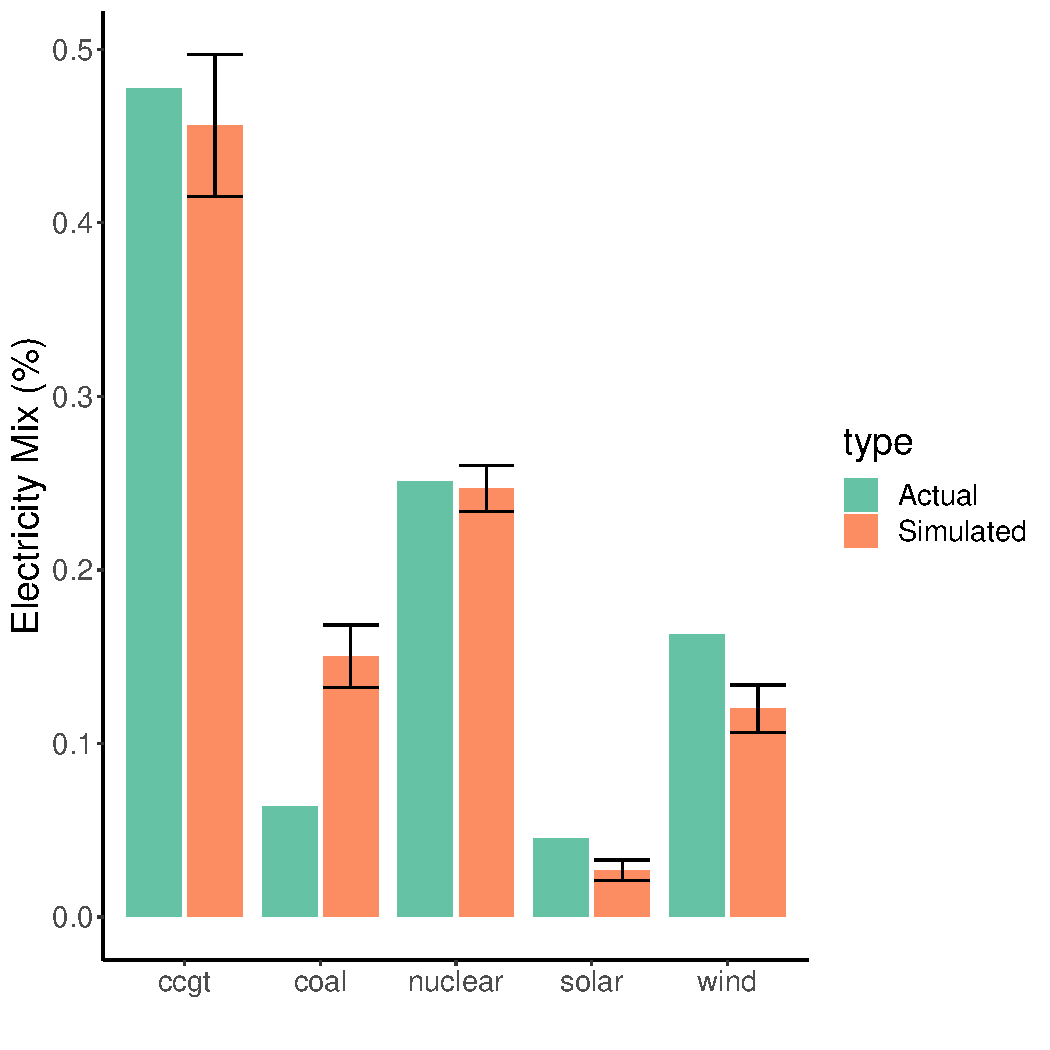
\includegraphics[width=0.46\textwidth]{figures/results/best_run.pdf}
\label{uk_historical_mix}
\caption{Electricity generation transition from 2013 to 2018 in the United Kingdom.}
\end{figure}

\begin{itemize}
	\item Clear and concise results
\end{itemize}

\section{Discussion}
\label{sec:discussion}

\begin{itemize}
	\item Significance of work
	\item Avoid discussion of public work
\end{itemize}

\section{Conclusion}
\label{sec:conclusion}

\begin{itemize}
	\item Main conclusions
\end{itemize}

\section{Funding Sources}

This work was supported by the Engineering and Physical Sciences Research Council, Centre for Doctoral Training in Cloud Computing for Big Data [grant number EP/L015358/1].




%% The Appendices part is started with the command \appendix;
%% appendix sections are then done as normal sections
%% \appendix

%% \section{}
%% \label{}

%% If you have bibdatabase file and want bibtex to generate the
%% bibitems, please use
%%
  \bibliographystyle{elsarticle-num} 
  \section*{References}
  \bibliography{library,bib_custom}

%% else use the following coding to input the bibitems directly in the
%% TeX file.

%\begin{thebibliography}{00}
%
%%% \bibitem[Author(year)]{label}
%%% Text of bibliographic item
%
%\bibitem[ ()]{}
%
%\end{thebibliography}
\end{document}

\endinput
%%
%% End of file `elsarticle-template-harv.tex'.
